\documentclass[border=8mm]{standalone}
\usepackage{tikz}
\usepackage[T1]{fontenc}
\usepackage{lmodern}

\begin{document}
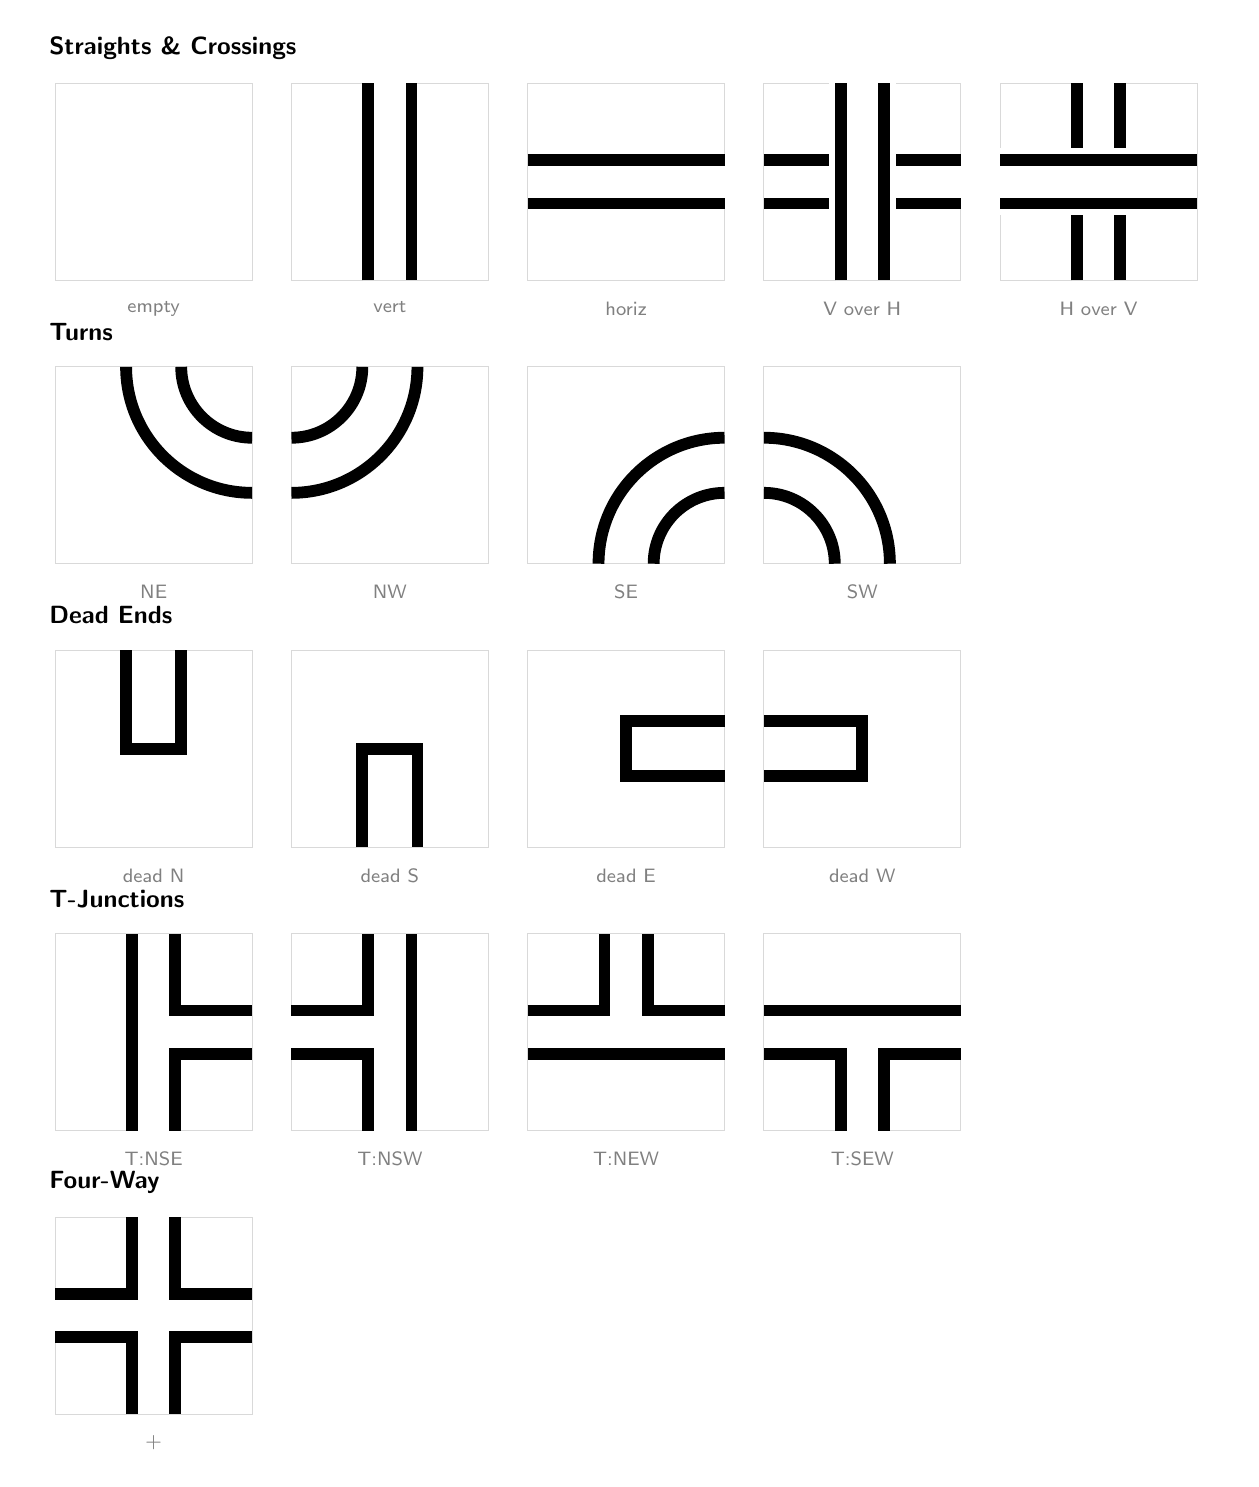
\begin{tikzpicture}[
  % Bordered ribbon: 7mm total, 1.5mm black edge each side, 4mm white interior
  o/.style={line width=7mm, draw=black, line cap=butt},
  i/.style={line width=4mm, draw=white, line cap=butt},
  % Crossing wipe
  w/.style={line width=8.5mm, draw=white, line cap=butt},
  % Explicit wall line (for turns and dead ends)
  wall/.style={line width=1.5mm, draw=black, line cap=butt, line join=miter},
  % Frame and labels
  bdr/.style={draw=black!15, line width=0.3pt},
  lbl/.style={font=\scriptsize\sffamily, text=black!50, anchor=north},
]

\def\S{2.5}    % tile size
\def\G{0.5}    % column gap
\def\RG{1.1}   % row gap
\def\R{1.25}   % half tile = corridor center radius
\def\HW{0.35}  % half corridor outer width (7mm/2 = 3.5mm = 0.35cm)
\def\Ri{0.9}   % inner wall radius = R - HW
\def\Ro{1.6}   % outer wall radius = R + HW

% ===== Row 0: Straights & Crossings =====
\node[font=\small\bfseries\sffamily, anchor=west] at (-0.2, \S+0.45) {Straights \& Crossings};

% empty
\begin{scope}[shift={(0,0)}]
  \draw[bdr] (0,0) rectangle (\S,\S);
  \node[lbl] at (\R,-0.15) {empty};
\end{scope}

% vert
\begin{scope}[shift={(\S+\G,0)}]
  \draw[bdr] (0,0) rectangle (\S,\S);
  \draw[o] (\R,0)--(\R,\S); \draw[i] (\R,0)--(\R,\S);
  \node[lbl] at (\R,-0.15) {vert};
\end{scope}

% horiz
\begin{scope}[shift={(2*\S+2*\G,0)}]
  \draw[bdr] (0,0) rectangle (\S,\S);
  \draw[o] (0,\R)--(\S,\R); \draw[i] (0,\R)--(\S,\R);
  \node[lbl] at (\R,-0.15) {horiz};
\end{scope}

% V over H
\begin{scope}[shift={(3*\S+3*\G,0)}]
  \draw[bdr] (0,0) rectangle (\S,\S);
  \draw[o] (0,\R)--(\S,\R); \draw[i] (0,\R)--(\S,\R);   % under: horiz
  \draw[w] (\R,0)--(\R,\S);                                % wipe
  \draw[o] (\R,0)--(\R,\S); \draw[i] (\R,0)--(\R,\S);     % over: vert
  \node[lbl] at (\R,-0.15) {V over H};
\end{scope}

% H over V
\begin{scope}[shift={(4*\S+4*\G,0)}]
  \draw[bdr] (0,0) rectangle (\S,\S);
  \draw[o] (\R,0)--(\R,\S); \draw[i] (\R,0)--(\R,\S);     % under: vert
  \draw[w] (0,\R)--(\S,\R);                                 % wipe
  \draw[o] (0,\R)--(\S,\R); \draw[i] (0,\R)--(\S,\R);      % over: horiz
  \node[lbl] at (\R,-0.15) {H over V};
\end{scope}

% ===== Row 1: Turns =====
% Fixed: two explicit wall arcs (inner + outer) instead of overlay,
% so passage ends remain open at tile edges.
\def\RowOne{-\S-\RG}
\node[font=\small\bfseries\sffamily, anchor=west] at (-0.2, \RowOne+\S+0.45) {Turns};

% NE — concave arc centered at NE corner (S,S), curving toward cell center
\begin{scope}[shift={(0,\RowOne)}]
  \draw[bdr] (0,0) rectangle (\S,\S);
  \draw[wall] ({\S-\Ri},\S) arc[start angle=180, delta angle=90, radius=\Ri cm];
  \draw[wall] ({\S-\Ro},\S) arc[start angle=180, delta angle=90, radius=\Ro cm];
  \node[lbl] at (\R,-0.15) {NE};
\end{scope}

% NW — concave arc centered at NW corner (0,S)
\begin{scope}[shift={(\S+\G,\RowOne)}]
  \draw[bdr] (0,0) rectangle (\S,\S);
  \draw[wall] (0,{\S-\Ri}) arc[start angle=270, delta angle=90, radius=\Ri cm];
  \draw[wall] (0,{\S-\Ro}) arc[start angle=270, delta angle=90, radius=\Ro cm];
  \node[lbl] at (\R,-0.15) {NW};
\end{scope}

% SE — concave arc centered at SE corner (S,0)
\begin{scope}[shift={(2*\S+2*\G,\RowOne)}]
  \draw[bdr] (0,0) rectangle (\S,\S);
  \draw[wall] (\S,\Ri) arc[start angle=90, delta angle=90, radius=\Ri cm];
  \draw[wall] (\S,\Ro) arc[start angle=90, delta angle=90, radius=\Ro cm];
  \node[lbl] at (\R,-0.15) {SE};
\end{scope}

% SW — concave arc centered at SW corner (0,0)
\begin{scope}[shift={(3*\S+3*\G,\RowOne)}]
  \draw[bdr] (0,0) rectangle (\S,\S);
  \draw[wall] (\Ri,0) arc[start angle=0, delta angle=90, radius=\Ri cm];
  \draw[wall] (\Ro,0) arc[start angle=0, delta angle=90, radius=\Ro cm];
  \node[lbl] at (\R,-0.15) {SW};
\end{scope}

% ===== Row 2: Dead Ends =====
% Fixed: U-shaped wall paths with flat closing bar, no circles.
\def\RowTwo{-2*\S-2*\RG}
\node[font=\small\bfseries\sffamily, anchor=west] at (-0.2, \RowTwo+\S+0.45) {Dead Ends};

% dead N — corridor enters from north, closes at center
\begin{scope}[shift={(0,\RowTwo)}]
  \draw[bdr] (0,0) rectangle (\S,\S);
  \draw[wall] ({\R-\HW},\S) -- ({\R-\HW},\R) -- ({\R+\HW},\R) -- ({\R+\HW},\S);
  \node[lbl] at (\R,-0.15) {dead N};
\end{scope}

% dead S — corridor enters from south, closes at center
\begin{scope}[shift={(\S+\G,\RowTwo)}]
  \draw[bdr] (0,0) rectangle (\S,\S);
  \draw[wall] ({\R-\HW},0) -- ({\R-\HW},\R) -- ({\R+\HW},\R) -- ({\R+\HW},0);
  \node[lbl] at (\R,-0.15) {dead S};
\end{scope}

% dead E — corridor enters from east, closes at center
\begin{scope}[shift={(2*\S+2*\G,\RowTwo)}]
  \draw[bdr] (0,0) rectangle (\S,\S);
  \draw[wall] (\S,{\R+\HW}) -- (\R,{\R+\HW}) -- (\R,{\R-\HW}) -- (\S,{\R-\HW});
  \node[lbl] at (\R,-0.15) {dead E};
\end{scope}

% dead W — corridor enters from west, closes at center
\begin{scope}[shift={(3*\S+3*\G,\RowTwo)}]
  \draw[bdr] (0,0) rectangle (\S,\S);
  \draw[wall] (0,{\R+\HW}) -- (\R,{\R+\HW}) -- (\R,{\R-\HW}) -- (0,{\R-\HW});
  \node[lbl] at (\R,-0.15) {dead W};
\end{scope}

% ===== Row 3: T-Junctions =====
\def\RowThree{-3*\S-3*\RG}
\node[font=\small\bfseries\sffamily, anchor=west] at (-0.2, \RowThree+\S+0.45) {T-Junctions};

% T:NSE
\begin{scope}[shift={(0,\RowThree)}]
  \draw[bdr] (0,0) rectangle (\S,\S);
  \draw[o] (\R,0)--(\R,\S); \draw[o] (\R,\R)--(\S,\R);
  \draw[i] (\R,0)--(\R,\S); \draw[i] (\R,\R)--(\S,\R);
  \node[lbl] at (\R,-0.15) {T:NSE};
\end{scope}

% T:NSW
\begin{scope}[shift={(\S+\G,\RowThree)}]
  \draw[bdr] (0,0) rectangle (\S,\S);
  \draw[o] (\R,0)--(\R,\S); \draw[o] (0,\R)--(\R,\R);
  \draw[i] (\R,0)--(\R,\S); \draw[i] (0,\R)--(\R,\R);
  \node[lbl] at (\R,-0.15) {T:NSW};
\end{scope}

% T:NEW
\begin{scope}[shift={(2*\S+2*\G,\RowThree)}]
  \draw[bdr] (0,0) rectangle (\S,\S);
  \draw[o] (0,\R)--(\S,\R); \draw[o] (\R,\R)--(\R,\S);
  \draw[i] (0,\R)--(\S,\R); \draw[i] (\R,\R)--(\R,\S);
  \node[lbl] at (\R,-0.15) {T:NEW};
\end{scope}

% T:SEW
\begin{scope}[shift={(3*\S+3*\G,\RowThree)}]
  \draw[bdr] (0,0) rectangle (\S,\S);
  \draw[o] (0,\R)--(\S,\R); \draw[o] (\R,0)--(\R,\R);
  \draw[i] (0,\R)--(\S,\R); \draw[i] (\R,0)--(\R,\R);
  \node[lbl] at (\R,-0.15) {T:SEW};
\end{scope}

% ===== Row 4: Four-Way =====
\def\RowFour{-4*\S-4*\RG}
\node[font=\small\bfseries\sffamily, anchor=west] at (-0.2, \RowFour+\S+0.45) {Four-Way};

% +
\begin{scope}[shift={(0,\RowFour)}]
  \draw[bdr] (0,0) rectangle (\S,\S);
  \draw[o] (\R,0)--(\R,\S); \draw[o] (0,\R)--(\S,\R);
  \draw[i] (\R,0)--(\R,\S); \draw[i] (0,\R)--(\S,\R);
  \node[lbl] at (\R,-0.15) {$+$};
\end{scope}

\end{tikzpicture}
\end{document}
